\chapter{Oscillator phase noise}


\section{Motivation}
An oscillator with negligible amplitude variation is well-described by
\begin{equation}
  A(t) = A_0 e^{i [\omega_0 t + \phi(t)]},
\end{equation}
where $\phi(t)$ is a zero-mean, stationary, random process
whose temporal variation causes
the oscillator's instantaneous frequency
to wander about its nominal value $\nu_0 = \omega_0 / (2 \pi)$.
The oscillator's phase change between
times $t$ and $t + \tau_j$ is
\begin{equation}
  \arg[A(t + \tau_j) \cdot A^*(t)]
  =
  \omega_0 \tau_j + \phi(t + \tau_j) - \phi(t).
\end{equation}
In a perfect oscillator,
$\phi(t + \tau_j) = \phi(t)$ for all $t$ and $\tau_j$
such that the phase change is governed only by
the oscillator's nominal frequency $\omega_0 / (2 \pi)$ and
the time difference $\tau_j$.
Excursions from this ideal result in phase noise.

It is the goal of this appendix
to investigate the spectral properties
of an oscillator's phase noise.
Define the phase noise between times $t$ and $t + \tau_j$ to be
\begin{equation}
  \delta \phi(t, \tau_j)
  \equiv
  \phi(t + \tau_j) - \phi(t).
\end{equation}
This phase noise can be related to
the deviation in the oscillator's instantaneous frequency via
\begin{equation}
  \delta \phi(t, \tau_j)
  =
  2 \pi \int_{t}^{t + \tau_j} \delta \nu(t') dt'.
  \label{eq:OscillatorPhaseNoise:phase_noise_from_frequency_deviation}
\end{equation}
Whereas the phase noise $\delta \phi(t, \tau_j)$
depends on the externally imposed time difference $\tau_j$,
the oscillator's instantaneous frequency deviation $\delta \nu(t)$ does not
(i.e.\ it is an intrinsic property of the oscillator).


\section{Autospectral density of phase noise}
The two-sided autospectral density $S_{xx}(f)$
of a stationary random process $\{x_k(t)\}$ is simply
\begin{equation}
  S_{xx}(f) = \mathcal{F}[R_{xx}(\tau)](f),
\end{equation}
where $\mathcal{F}$ is the Fourier transform operator and
$R_{xx}(\tau)$ is the autocorrelation of $\{x_k(t)\}$
\cite[Sec.~5.2.1]{bendat_and_piersol}.
Below, the phase-noise autocorrelation
$R_{\delta\phi,\delta\phi}(\tau)$ is computed;
subsequently, the phase-noise autospectral density
$S_{\delta\phi,\delta\phi}(f)$ is computed
by Fourier transforming
$R_{\delta\phi,\delta\phi}(\tau)$.


\subsection{Autocorrelation of phase noise}
The autocorrelation $R_{xx}(\tau)$
of a stationary random process $\{x_k(t)\}$ is defined as
\begin{equation}
  R_{xx}(\tau) = E\left[ x_k(t) x_k(t + \tau) \right],
\end{equation}
where $E$ is the expectation-value operator
that averages over all of the realizations in the ensemble $\{x_k(t)\}$
\cite[Sec.~5.1.1]{bendat_and_piersol}.
Note that the autocorrelation of a stationary process
is an \emph{even} function:
$R_{xx}(-\tau) = R_{xx}(\tau)$.

Using the above definition,
the phase noise
(\ref{eq:OscillatorPhaseNoise:phase_noise_from_frequency_deviation})
has an autocorrelation
\begin{align}
  R_{\delta\phi,\delta\phi}(\tau)
  &=
  E\left[ \delta\phi(t) \delta\phi(t + \tau) \right]
  \notag \\
  &=
  (2 \pi)^2
  \int_{t}^{t + \tau_j} dt'
  \int_{t + \tau}^{t + \tau + \tau_j} dt'' \,
  E[ \delta \nu(t') \delta \nu(t'') ],
  \label{eq:OscillatorPhaseNoise:phase_noise_autocorrelation_v1}
\end{align}
where the linearity of the expectation-value operator has been used
to bring $E$ into the integrand of the double integral.
Note that
$E[ \delta \nu(t') \delta \nu(t'') ]
=
R_{\delta\nu,\delta\nu}(t', t'')
=
R_{\delta\nu,\delta\nu}(t' - t'')$, where
the last equality follows from the fact that
the autocorrelation of a stationary process
cannot depend on the absolute times $t'$ and $t''$
\emph{except} through their difference $t' - t''$.
Thus, (\ref{eq:OscillatorPhaseNoise:phase_noise_autocorrelation_v1})
becomes
\begin{equation}
  R_{\delta\phi,\delta\phi}(\tau)
  =
  (2 \pi)^2
  \int_{t}^{t + \tau_j} dt'
  \int_{t + \tau}^{t + \tau + \tau_j} dt'' \,
  R_{\delta\nu,\delta\nu}(t' - t'').
  \label{eq:OscillatorPhaseNoise:phase_noise_autocorrelation_v2}
\end{equation}

Fortunately, a suitable change of variables
simplifies the expression for
$R_{\delta\phi,\delta\phi}(\tau)$ in
(\ref{eq:OscillatorPhaseNoise:phase_noise_autocorrelation_v2}).
To see this, define the integral
\begin{equation}
  I(g, \tau, \tau_j)
  \equiv
  \int_{a}^{a + \tau_j} dx
  \int_{a + \tau}^{a + \tau + \tau_j} dy \,
  g(x - y),
\end{equation}
and make the change of variables
\begin{equation}
  x = z + y,
  \label{eq:OscillatorPhaseNoise:change_of_variables}
\end{equation}
which transforms the integration domain as shown in
Fig.~\ref{fig:OscillatorPhaseNoise:integration_domains}.
Then, $I(g, \tau, \tau_j)$ becomes
\begin{align}
  I(g, \tau, \tau_j)
  &=
  \int_{- \tau_j - \tau}^{- \tau} dz \, g(z)
  \int_{a - z}^{a + \tau + \tau_j} dy
  +
  \int_{-\tau}^{\tau_j - \tau} dz \, g(z)
  \int_{a + \tau}^{a + \tau_j - z} dy
  \notag \\
  &=
  \int_{- \tau_j - \tau}^{- \tau} dz \,
  \left[ \tau_j + (z + \tau) \right]
  g(z)
  +
  \int_{-\tau}^{\tau_j - \tau} dz \,
  \left[ \tau_j - (z + \tau) \right]
  g(z)
  \notag \\
  &=
  \int_{-\tau_j}^{0} dz' \,
  \left[ \tau_j + z' \right]
  g(z' - \tau)
  +
  \int_{0}^{\tau_j} dz' \,
  \left[ \tau_j - z' \right]
  g(z' - \tau)
  \notag \\
  &=
  \int_{-\tau_j}^{\tau_j} dz' \,
  \left[ \tau_j - |z'| \right]
  g(z' - \tau)
  \label{eq:OscillatorPhaseNoise:integral_after_change_of_variables}
\end{align}
Substituting (\ref{eq:OscillatorPhaseNoise:integral_after_change_of_variables})
into (\ref{eq:OscillatorPhaseNoise:phase_noise_autocorrelation_v2})
with $g = R_{\delta\nu,\delta\nu}$ and
using the fact that the autocorrelation is even
yields
\begin{equation}
  R_{\delta\phi,\delta\phi}(\tau)
  =
  (2 \pi)^2
  \int_{-\tau_j}^{\tau_j} dt' \,
  \left[ \tau_j - |t'| \right]
  R_{\delta\nu,\delta\nu}(\tau - t').
  \label{eq:OscillatorPhaseNoise:phase_noise_autocorrelation_final}
\end{equation}

\begin{figure}
  \centering
  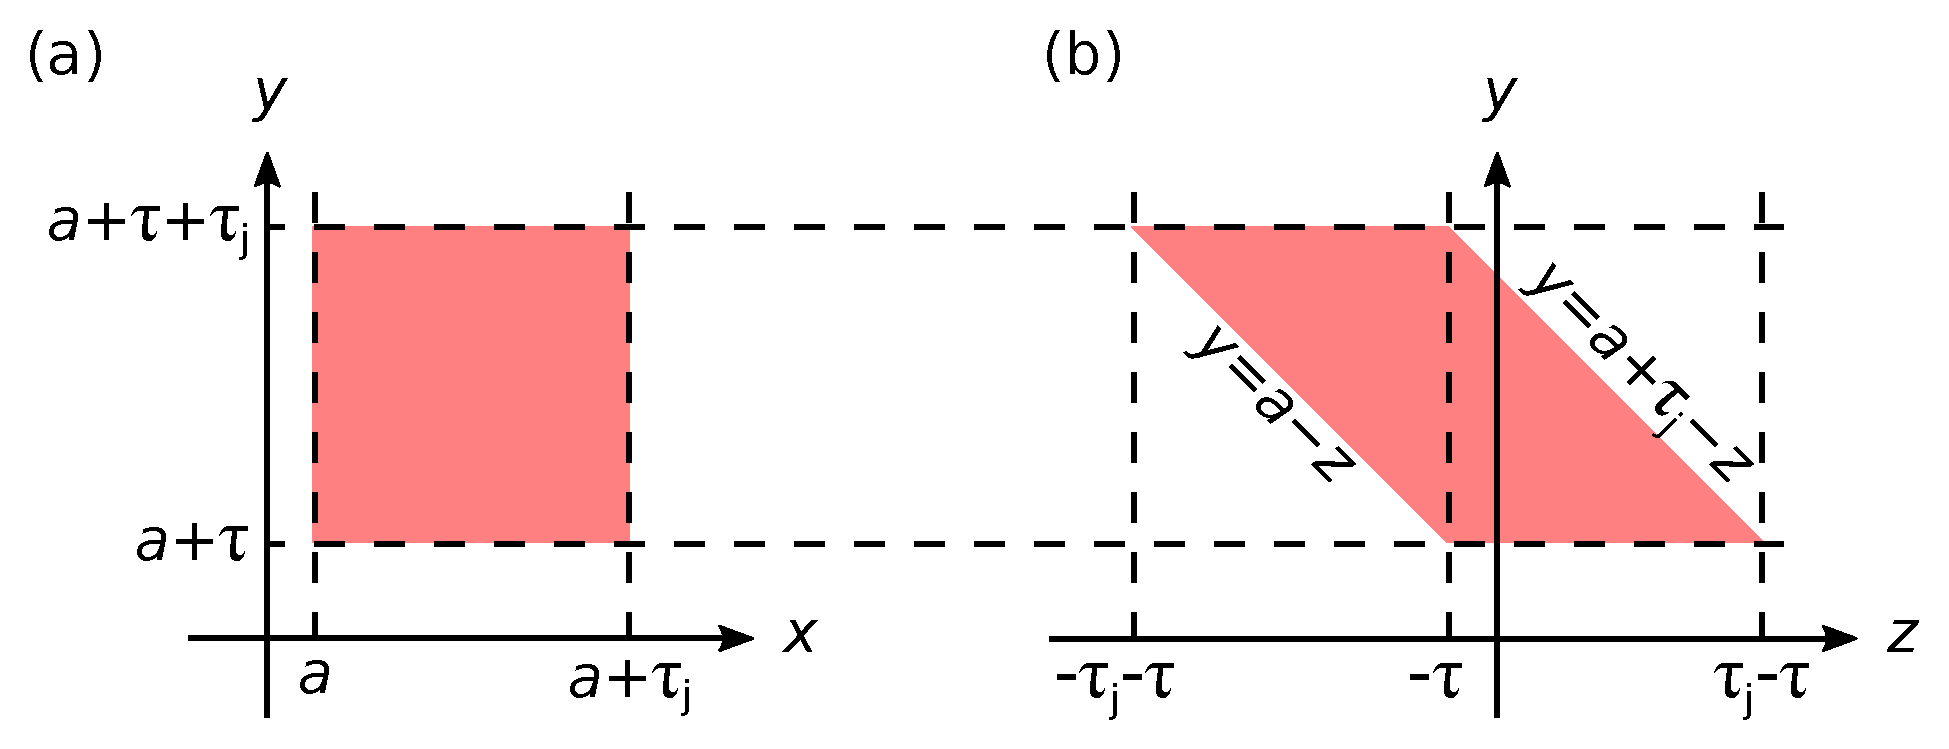
\includegraphics[width = \textwidth]{%
    Appendices/OscillatorPhaseNoise/figs/integration_domains.pdf}
  \caption[Integration domains]{
    Integration domains (a) before and (b) after
    the change of variables in
    (\ref{eq:OscillatorPhaseNoise:change_of_variables}).}
  \label{fig:OscillatorPhaseNoise:integration_domains}
\end{figure}


\subsection{Autospectral density of phase noise}
Taking the Fourier transform of
the phase-noise autocorrelation
(\ref{eq:OscillatorPhaseNoise:phase_noise_autocorrelation_final})
yields the phase-noise autospectral density
\begin{align}
  S_{\delta\phi,\delta\phi}(f)
  &=
  \mathcal{F}
  \left[%
    R_{\delta\phi,\delta\phi}(\tau)
  \right](f)
  \notag \\
  &=
  (2 \pi)^2
  \int_{-\tau_j}^{\tau_j} dt' \,
  \left[ \tau_j - |t'| \right]
  \mathcal{F}
  \left[
    R_{\delta\nu,\delta\nu}(\tau - t')
  \right](f)
  \notag \\
  &=
  (2 \pi)^2 \,
  S_{\delta\nu,\delta\nu}(f)
  \int_{-\tau_j}^{\tau_j} dt' \,
  \left[ \tau_j - |t'| \right]
  e^{i 2 \pi f t'}
  \notag \\
  &=
  [2 \pi \tau_j \sinc(f \tau_j)]^2 \,
  S_{\delta\nu,\delta\nu}(f)
  \label{eq:OscillatorPhaseNoise:phase_noise_autospectral_density}
\end{align}
where the Fourier transform's
linear and translational properties have been used and
$\sinc(x) = \sin(\pi x) / (\pi x)$ is the normalized sinc function.
Now, if $f \tau_j \ll 1$, as is often of practical relevance,
\begin{equation}
  S_{\delta\phi,\delta\phi}(f)
  \approx
  [2 \pi \tau_j]^2 \,
  S_{\delta\nu,\delta\nu}(f);
  \label{eq:OscillatorPhaseNoise:phase_noise_autospectral_density_approx}
\end{equation}
that is, an oscillator's phase-noise autospectral density is
linearly related to the autospectral density
of the oscillator's underlying frequency deviation
(an intrinsic property of the oscillator) and
quadratically related to the temporal duration $\tau_j$.


\bibliographystyle{plainurl}
\bibliography{references}
